%!TEX root = ../thesis.tex

\renewcommand\thefigure{\thechapter.\arabic{figure}}
\renewcommand{\thesection}{\thechapter.\arabic{section}}
\normalsize


\thispagestyle{empty}

\begin{tikzpicture}[remember picture,overlay]
\node at (current page.center) {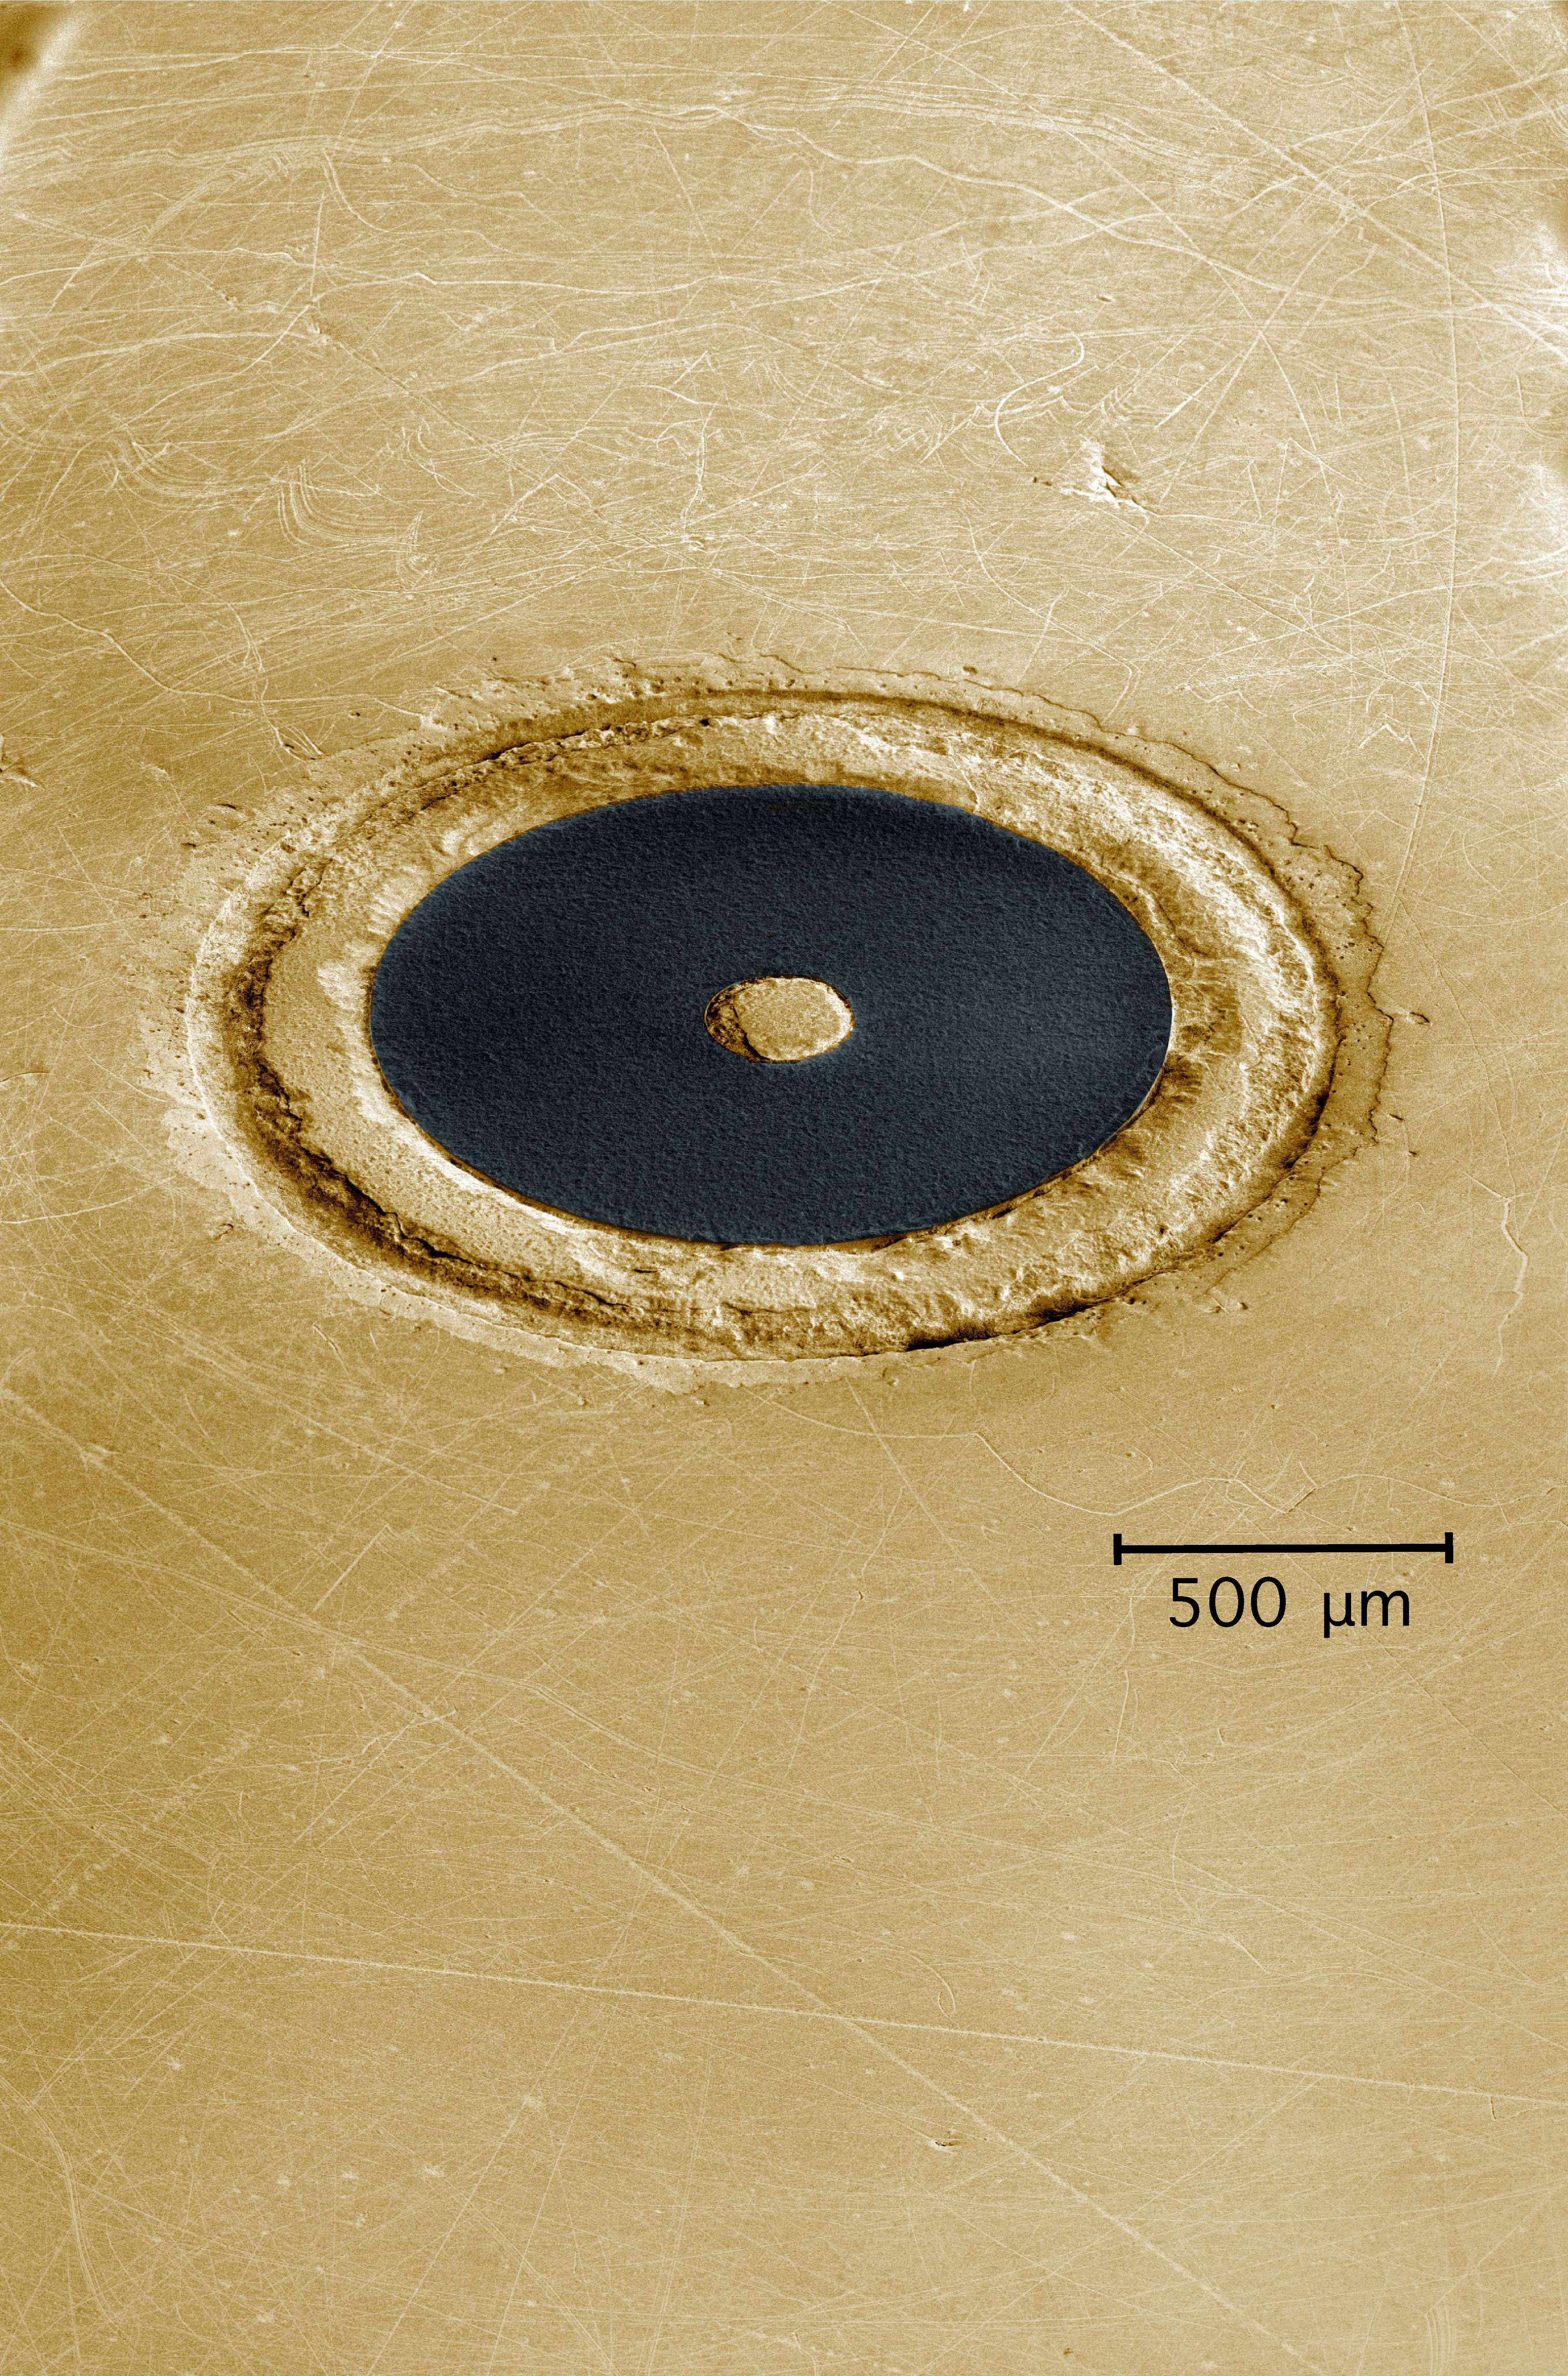
\includegraphics[width=\pdfpagewidth,height=\pdfpageheight]{fullpage_images/Head_SampleCell.pdf}};
\end{tikzpicture}

\clearpage



\begin{savequote}[75mm]
$\blacktriangleleft$ Top view of the coaxial-probe head used for dielectric relaxation measurements. The marks on the surface show the erosion caused throughout the experiments presented in Chapters 4--6.

\vspace{3pt}

SEM Photo, Lukas Helmbrecht. Edition, Roberto Cota
\end{savequote}




%\chapter{Dielectric relaxation spectroscopy\myfnt{{\it Sections~\ref{FormalismSection} and ~\ref{sec:VSFG-methods} of this chapter are based on:} S. J. Roeters, C. N. van Dijk, A. Torres-Knoop, E. H. G. Backus, R. K. Campen, M. Bonn, and S. Woutersen, \textit{The Journal of Physical Chemistry A} \textbf{117} (29), pp. 6311–6322 (2013).}}



\chapter[Methods I: Dielectric relaxation spectroscopy]{Methods I\\Dielectric relaxation spectroscopy}
\label{chap:methods1}
\label{MethodsChapter2}
\label{ChapterDRS}

\vspace{30pt}


The polarization properties of aqueous solutions, intimately linked to molecular structuring and solvation properties, are discussed in this chapter. First, we introduce the concept of dipole moment reorientation that results from the interaction with external electric fields. Then, we provide the microscopic molecular description underlying the observed macroscopic dielectric properties. As such, we can use dielectric relaxation spectroscopy to study molecular mobility and molecular cooperativity. If electrolyte solutions are our samples of interest, we can determine the extent to which ions affect the hydrogen bonding interactions of water. The discussion on the local ordering effect of water molecules in solvation shells is also one of the main goals of this chapter. Finally, the data analysis and modeling of the dielectric relaxation measurements are described.



\newpage



\section{Electromagnetic waves interacting with matter}\label{MolVibs}

A complete (classical) description of propagating electromagnetic fields can be performed by means of the Maxwell equations\!\cite{Jackson1999}
\begin{eqnarray}
\nabla \cdot \vec{D} &=& \rho_e, \label{GaussLaw} \\
\nabla \cdot \vec{B} &=& 0, \label{MagGaussLaw} \\
\nabla \times \vec{E} &=& - \frac{\partial \vec{B}}{\partial t}, \label{FaradayLaw} \\
\nabla \times \vec{H} &=& \vec{j} + \frac{\partial \vec{D}}{\partial t}, \label{AmpereLaw}
\end{eqnarray}
\noindent in which Eq.\ \ref{GaussLaw} shows that the electric displacement $\vec{D}$ is determined by the distribution of electric charges $\rho_e$. Gauss's law for magnetism, Eq.\ \ref{MagGaussLaw}, states that the net magnetic field $\vec{B}$ over a closed surface must be zero, meaning that magnetic monopoles cannot exist. The Maxwell-Faraday equation, Eq.\ \ref{FaradayLaw} describes the induction of electric fields as the result of time-varying magnetic fields. While Amp\`ere's law, Eq.\ \ref{AmpereLaw}, indicates the induced magnetic fields due to electrical currents and time-varying electric fields. 


For an homogeneous and isotropic material with intrinsic properties that are time-independent, one can derive the following three constitutive equations
\begin{eqnarray}
\vec{D} &=& \epsilon_0 \vec{E} + \vec{P} = \epsilon_0 \hat{\epsilon} \vec{E}, \label{DtoE} \\
\vec{B} &=& \mu_0 \vec{H} + \vec{M} = \mu_0 \hat{\mu} \vec{H}, \label{HtoB} \\
\vec{j} &=& \kappa \vec{E}, \label{ConduConstitutive}
\end{eqnarray}
\noindent where $\vec{P}$ and $\vec{M}$ are the polarization and magnetization density vectors, respectively. The material properties are described by the complex relative electric permittivity $\hat{\epsilon}$ and the complex relative magnetic permeability $\hat{\mu}$. These properties can also be expressed with the electric and magnetic susceptibilities of the material as $\hat{\epsilon} = 1 + \hat{\chi}_e$ and $\hat{\mu} = 1 + \hat{\chi}_m$. The quantities $\epsilon_0$ and $\mu_0$ describe the permittivity and permeability of free space. The quantity $\kappa$ is the specific conductivity of the material. It is important to notice that Eqs.\ \ref{GaussLaw}-\ref{ConduConstitutive} constitute a set of linear equations to compute all kind of electromagnetic interactions.



From Eq.\ \ref{DtoE}, one can observe that the electric displacement results from the polarization response of the material due to electric forces. This polarization response can involve  a displacement of the electron cloud of atoms or molecules with respect of the unperturbed state. It can also involve the reorientation of a dipolar molecular towards the direction of the electric field $\vec{E}$. In the case of static electric fields, the complex permittivity reduces to the so-called static permittivity $\epsilon_\text{s}$, which is also commonly referred to as dielectric constant. The latter quantity defines the total static polarization. 



Due to microscopic interactions and inertial effects, the reaction of the medium to an applied external electric field is not instantaneous. Instead, the system requires a time interval to reorient following the direction of the external field, meaning that the polarization effect is delayed with respect to the electric field $\vec{E}$. If we consider a monochromatic oscillating electric field $\vec{E}(t) = \vec{E}_0 cos (\omega t)$ with amplitude $\vec{E}_0$, a phase shift between $\vec{D}$ and $\vec{E}$ will emerge that depends on the frequency $\omega$:
\begin{eqnarray}
\vec{D} (t) = \vec{D}_0 \cos [\omega t -\delta (\omega)],
\label{DisplacementDelay1}
\end{eqnarray}
\noindent with $\delta(\omega)$ the frequency-dependent phase delay, which is also referred to as loss angle. Notice that $\vec{D}_0 = \epsilon_0 \hat{\epsilon}(\omega) \vec{E}_0$ according to Eq.\ \ref{DtoE}.



By introducing the following reciprocal representation in the complex plane
\begin{eqnarray}
\vec{D}_0 [\cos \delta - i \sin \delta ] = \epsilon_0 \vec{E}_0 [\epsilon' - i \epsilon''],
\end{eqnarray}
\noindent the electric displacement given in Eq.\ \ref{DisplacementDelay1} can be expressed with the following formula
\begin{eqnarray}
\vec{D} (t) = \epsilon'(\omega) \epsilon_0 \vec{E}_0 \cos(\omega t) +  \epsilon'' (\omega) \epsilon_0 \vec{E}_0 \sin(\omega t).
\label{DisplacementDelay2}
\end{eqnarray}



The preceding equation shows that the electric displacement arises from two effects with different nature: (i) the in-phase dielectric dispersion is proportional to the real part of the relative permittivity, while (ii) the out-of-phase dielectric dissipation (dielectric loss) is proportional to the imaginary part of the relative permittivity. It is clear from Eq.\ \ref{DisplacementDelay2} that the mathematical formulation can be promoted to complex notation, i.e.\ $ \hat{\vec{D}} = \epsilon_0 \hat{\epsilon} \hat{\vec{E}}$. Notice that a similar delayed response can occur between the magnetic flux $\vec{B}$ and the magnetic field strength $\vec{H}$, and therefore Eq.\ \ref{HtoB} can be analogously written as Eq.\ \ref{DisplacementDelay2}.



One can describe the evolution of the electromagnetic fields as plane waves with the following functional forms
\begin{eqnarray}
\hat{\vec{E}} (\vec{r},t) &=& \hat{\vec{E}} (\vec{r}) \exp (i \omega t),\\
\hat{\vec{H}} (\vec{r},t) &=& \hat{\vec{H}} (\vec{r}) \exp (i \omega t),
\label{harmonicoscillators}
\end{eqnarray}
\noindent which in combination of Eqs.\ \ref{GaussLaw}--\ref{ConduConstitutive} (with a net electric charge of zero, i.e\ $\nabla \cdot \vec{D} = 0$) lead to the following wave equations
\begin{eqnarray}
\nabla^2 \hat{\vec{E}} (\vec{r}) + \hat{k}^2 \hat{\vec{E}} (\vec{r}) &=& 0 ,
\label{helmholtzeq1}
\\ \nabla^2 \hat{\vec{H}} (\vec{r}) + \hat{k}^2 \hat{\vec{H}} (\vec{r}) &=& 0,
\label{helmholtzeq2}
\end{eqnarray}
\noindent that describe the propagation of electromagnetic waves through a material. A solution to Eq.\ \ref{helmholtzeq1} is given by $\vec{E} (\vec{r}) = E_0 \exp(i \vec{k} \cdot \vec{r})$, where $\hat{k}$ is the wave vector expressed by 
\begin{eqnarray}
\hat{k}^2 = k_0^2 \left[ \hat{\mu} (\omega) \hat{\epsilon} (\omega) + \frac{\hat{\mu} (\omega)  \hat{\kappa} (\omega)} {i \omega \epsilon_0}   \right].
\label{wavenumberP}
\end{eqnarray}
\noindent with $k_0 (= \omega \sqrt{\mu_0 \epsilon_0} = \omega/c  )$ the propagation constant in vacuum. The preceding equation describes the response of a medium to electromagnetic fields, and shows the extent to which the propagation of the field deviates from that observed in free space.


For electrolyte solutions, which are the focus of interest in this work, the wave vector can be written as
\begin{eqnarray}
\hat{k}^2 = k_0^2 \left[ \hat{\epsilon} (\omega) + \frac{  \sigma} {i \omega \epsilon_0}   \right],
\label{wavenumberP2}
\end{eqnarray}
\noindent where $\hat{\kappa} (\omega)$ reduces to the DC ionic conductivity $\sigma$, since its frequency dependence is irrelevant in the frequency range of our interest ($\sim$18 GHz the characteristic dielectric relaxation mode of water).\!\cite{Ghowsi1989,Anderson1994a,Ellison1996,Buchner1999b}

In electrolyte solutions, the energy loss (imaginary part) arises from the non-instantaneous rearrangement of charges in the dielectric medium, as well as from the work exerted by rotating dipoles. The real part of the dielectric dispersion is related to the temporarily stored energy, and determined by the degree of orientation of the dipoles along the direction of the electric field.


% $\hat{\kappa}$ reduces to the DC ionic conductivity $\sigma$, since the frequency-dependent character of $\hat{\kappa}$ is irrelevant in the frequency range of our interest ($\sim$~20 GHz the characteristic dielectric relaxation mode of water)~\cite{Ghowsi1989,Anderson1994a,Buchner1999b}. 







\section{Polarization}



The polarization of a medium can be defined as the net macroscopic dipole per volume of a medium in the presence of an electric field. From Eq.\ \ref{DtoE}, one can write
\begin{eqnarray}
\hat{\vec{P}} = (\hat{\epsilon} - 1) \epsilon_0  \hat{\vec{E}},
\label{polarizationvector}
\end{eqnarray}
\noindent in which the polarization is described as the dielectric response of the medium to $\hat{\vec{E}}$. The underlying microscopic definition can be understood as the sum of two contributions
\begin{eqnarray}
\hat{\vec{P}} = \hat{\vec{P}}_\mu + \hat{\vec{P}}_\alpha
\label{polarizationvectorSeparation}
\end{eqnarray}
where $\hat{\vec{P}}_\mu$ refers to the orientational response of molecular dipoles, while $\hat{\vec{P}}_\alpha$ is attributed to the polarization resulting from the intramolecular polarizability. 





These two contribution are generally well separated. The orientational relaxation of dipoles along the applied electric field typically takes place in the order of picoseconds or slower, such as the dielectric response of water with a time constant of $\sim$8 ps at room temperature. While the molecular polarizability takes place at the femtosecond timescale. Thus, $\hat{\vec{P}}_\mu$ and $\hat{\vec{P}}_\alpha$ are considered independent with each other, leading to
\begin{eqnarray}
\hat{\vec{P}}_\mu = \epsilon_0 (\hat{\epsilon} - \epsilon_\infty) \hat{\vec{E}} \label{separationPolarization1}, \qquad \text{and} \qquad \hat{\vec{P}}_\alpha = \epsilon_0 (\epsilon_\infty - 1) \hat{\vec{E}},
\label{separationPolarization2}
\end{eqnarray}
\noindent with $\epsilon_\infty$ the permittivity in the intermediate frequency region at which dipoles are insensitive to the fast oscillating field, but the molecular polarizability has attained its maximum amplitude. Experiments focused on the dipolar orientation effect in aqueous solutions have shown that $\epsilon_\infty$ is constant in the GHz frequency region.\!\cite{Lileev2007} In the limit of a static electric field ($\omega \to 0$), the orientational polarization reduces to $\vec{P}_{\mu,0} = \epsilon_0 ( \epsilon_{\text{s}} - \epsilon_\infty) \vec{E}_0 $. The static permittivity $\epsilon_\text{s}$ is attained when all types of polarizations reach equilibrium with a switched-on DC electric field. The microscopic description is discussed in the following section.



\section{Microscopic description of static permittivity}



The macroscopic static permittivity can be connected to the microscopic notion of the collection of molecular dipoles aligned along the direction of the external field. 



Under the action of an electric field, dipoles tend to reorient towards the direction of the electric field in order to minimize their internal energy, defined as
\begin{eqnarray}
U (\theta) = - \vec{\mu} \cdot \vec{E} = - \mu E \cos{\theta},
\label{PotentialPolarization}
\end{eqnarray} 
where $\theta$ represents the angle between the dipole moment vector $\vec{\mu}$ and the electric field vector $\vec{E}$. Thus, it is clear to see that the minimum energy is attained at $\theta=0$, which mean a perfect alignment to the electric field. Such a situation is physically unaccessible since it means a system in perfect order with no entropy--this could theoretically occur at extremely low temperatures at which, ironically, the molecules would not have enough energy to rotate and align with the electric field. At non-zero temperatures the molecules will diffuse and rotate constantly because of the thermal energy of the system. 



Under the action of an external electric field, the orientation of the dipoles is slightly shifted from the random distribution, leading to an effective (averaged) dipole moment $\langle \vec{\mu} \rangle$. If we assume that the medium is formed by only one type of dipoles, the polarization can be written as
\begin{eqnarray}
\vec{P} = \rho \langle \vec{\mu} \rangle,
\label{GeneratlPolarization}
\end{eqnarray} 
which is proportional to the density $\rho$ of dipolar molecules.



In this view, the system is formed by dipoles with a statistical distribution between $\theta_\text{min} = 0 $ and $\theta_\text{max} = \pi$. The Boltzmann distribution equation can be used to determine the fraction of dipoles with a certain energy $U$:
\begin{eqnarray}
N (U) = A \exp \left( - \frac{U(\theta)} {k_\text{B} T} \right) 
\label{BoltzmannDistri}
\end{eqnarray} 
with $T$ and $k_\text{B}$ the temperature of the system and the Boltzmann constant, respectively. Given the preceding equation, the averaged dipole moment can be obtained summing up the contribution of all possible states, as follows
\begin{eqnarray}
\langle \vec{\mu} \rangle = \frac{ \int_0^\pi N[U(\theta)] \cdot \mu \cos \theta \cdot d\Omega     } {   \int_0^\pi N[U(\theta)] \cdot d\Omega   }
\label{AveragedMoment1}
\end{eqnarray} 
\noindent where $d\Omega$ ($= 2\pi \sin\theta d\theta$) is the solid angle increment on a unit sphere when $\theta$ changes to $\theta + d \theta$. Notice that $\Omega$ account for the three-dimensional system, in which the polarization is invariant to rotations over the azimuthal angle around the electric field vector. The solution to Eq.\ \ref{AveragedMoment1} yields $\langle \vec{\mu} \rangle = \mu \text{L}(\xi)$, with $\text{L}$ the Langevin equation, and $\xi = \mu E/ k_\text{B} T$. In the limit of $\xi \ll 1$ (which is valid even for very strong electric fields and strong dipoles), $\text{L} (\xi) \simeq \xi/3 $, we reach to the Langevin-Debye equation for the induced polarization is obtained\!\cite{DebyeBook1929,Evans1982}
\begin{eqnarray}
\vec{P} = \frac{\rho \mu^2}{3 k_\text{B} T} \vec{E} = \epsilon_0 (\epsilon_\text{s} - \epsilon_\infty) \vec{E},
\label{LangeDebyePolarization}
\end{eqnarray} 
and thus:
\begin{eqnarray}
\epsilon_\text{s} - \epsilon_\infty = \frac{\rho \mu^2}{3 \epsilon_0 k_\text{B} T}.
\label{FirstDielectricConstant}
\end{eqnarray} 



\subsection{The Lorentz cavity field and Debye's theory of dielectrics}



The above description assumes that each molecule is solely affected by the action of the external field, and the total polarization is the result of the collection of individual contributions. However, a dipole immerse in the system will be also affected by the macroscopic polarization of the system $\vec{P}$. The force that a given polar molecules experiences arises from the sum of the external field and the collective polarization of the system, such that 
\begin{eqnarray}
\vec{E}_\text{loc} = \vec{E} + \frac{\vec{P}}{3 \epsilon_0} \qquad \Longrightarrow \qquad \vec{E}_\text{loc} = \frac{\epsilon_\text{s} + 2}{3} \vec{E},
\label{LorentzField}
\end{eqnarray} 
which is known as the Lorentz cavity field.\!\cite{Lorentz1916} In this approach, one assumes that each dipole is inside a small spherical cavity with a charge distribution at the surface as the result of the macroscopic polarization. As can be seen in Eqs.\ \ref{GeneratlPolarization} and \ref{LorentzField}, the Lorentz field acts parallel to the applied field $\vec{E}$ and effectively enhances the response of the dipoles. 



Debye was the first one to use this notion to model the temperature-dependent dielectric constant, which Eq.\ \ref{FirstDielectricConstant} failed to predict. With this approach Debye derived
\begin{eqnarray}
\frac{\epsilon_\text{s} - 1}{\epsilon_\text{s} + 2} = \frac{\rho \mu^2}{9 \epsilon_0 k_\text{B} T} + \frac{\rho \alpha}{3 \epsilon_0},
\label{DebyeDielectricConstant}
\end{eqnarray} 
or if we consider the Clausius-Mossotti relation for molecular polarizability $\alpha$,\!\cite{choy1999effective} the dielectric constant can be written as
\begin{eqnarray}
\frac{\epsilon_\text{s} - 1}{\epsilon_\text{s} + 2} - \frac{\epsilon_\infty - 1}{\epsilon_\infty + 2} = \frac{\rho \mu^2}{9 \epsilon_0 k_\text{B} T},
\label{DebyeDielectricConstant2}
\end{eqnarray} 
which is limited to estimate the dielectric response of gases and dilute solutions of polar molecules in non-polar solvents due to assumptions in defining Eq.\ \ref{LorentzField}. %In this framework the central dipole is affected by the resultant field from neighbouring polar molecules, while the field generated by the central dipole is assumed negligible. This means that the medium is not influenced by the presence of the cavity, which is not entirely valid.  



Furthermore, if the term for polarizability is neglected, one can derive a critical behavior for the dielectric constant with the following functional form
\begin{eqnarray}
\epsilon_\text{s} = \frac{T + 2 T_c}{T - T_c}, \qquad \text{with} \qquad T_c = \frac{\rho \mu^2}{9 \epsilon_0 k_\text{B}},
\label{DebyeCritical}
\end{eqnarray} 
that defines a critical temperature $T_c$ at which the dielectric response would diverge. Near $T_c$, the polarization becomes so large, meaning extremely large local electric fields, that the dipoles would align to one another even in case of $E \sim 0$ (analogous to a permanent magnet!). This problem and limitations were spotted and criticized by Onsager.~\footnote{Onsager submitted a paper with a criticism of Debye's theory to \textit{Physikalische Zeitschrift} at which Debye was the editor by the time. It got rejected.\!\cite{ChristopherLonguet-Higgins1995}} Onsager derived a more strict model by noting that for dipolar molecules the local electric field differs from the average electric field that results from the polarization of all molecules in the medium.



\subsection{Onsager equation of dielectrics}



Onsager described the dielectric response as the contribution of polar molecules contained in spherical cavities with radius $a$, in which the sum of all the spheres equals to the volume of the material.\!\cite{Onsager1936,BOTTCHER1973} He started by computing the electric field in a spherical cavity resulting from the applied field in the dielectric medium surrounding the cavity, and the electric field resulting from the back reaction of the medium on the dipole moment of the molecule in the cavity.


%He started by computing the field produced by the dipole inside and outside the sphere, in which boundary conditions should be satisfied. Hence, Onsager's theory considers that the outer medium is affected by the presence of the polar cavity.



Within this model, the internal field acting on a given dipole consist of two contributions: (i) the cavity field generated which is parallel to the external field, and (ii) the reaction field resulting from the back reaction of the surrounding medium to the dipole in the cavity. Under the influence of these two fields, the confined dipole will be polarized so that its instantaneous dipole moment differs from its permanent dipole moment $\vec{\mu}$.\!\cite{Wilson1939}



Onsager was able to establish the following relation between dielectric constant, polarizability and vacuum dipole moment:
\begin{eqnarray}
\frac{ (\epsilon_\text{s} - \epsilon_\infty)   (2 \epsilon_\text{s} + \epsilon_\infty)    }{\epsilon_\text{s} (\epsilon_\infty +2)^2  } = \frac{\rho \mu^2}{9 \epsilon_0 k_\text{B} T},
\label{OnsagerDielectricConstant2}
\end{eqnarray}
which does not contain singularities, in contrast to Debye's description. This equation offers a better description for the dielectric constant of polar liquids.\!\cite{Wilson1939,Buchner1999b,Buchner1999}



\subsection{Kirkwood-Fr\"ohlich equation of dielectrics}\label{KirkFrohSection}


In the approaches of Debye and Onsager, the dielectric response has been established based on a continuum description of the dielectric medium, but the effect of intermolecular interactions has been neglected. Aqueous systems, which are of our interest, tend to behave in a cooperative manner. Kirkwood and later Fr\"ohlich performed a rigorous statistical study of the intermolecular interactions to extend the Onsager equation of dielectrics.\!\cite{Kirkwood1939a,BOTTCHER1973,Frohlich1986} They derived the following expression
\begin{eqnarray}
\frac{ (\epsilon_\text{s} - \epsilon_\infty)   (2 \epsilon_\text{s} + \epsilon_\infty)    }{\epsilon_\text{s} (\epsilon_\infty +2)^2  } = \frac{\rho \mu^2 g_\text{K}}{9 \epsilon_0 k_\text{B} T},
\label{KirkFroConstant}
\end{eqnarray}
\noindent where $g_\text{K}= 1 + z \langle \cos \gamma \rangle$ is the Kirkwood correlation factor which is a measure of the microscopic ordering of the medium. In the latter expression for $g_\text{K}$, $z$ is the solvation number and $\langle \cos \gamma \rangle$ is the average orientation between two neighbouring dipoles. Notice that in the limit $g_\text{K} = 1$, which corresponds to a completely uncorrelated orientation of the dipoles, Eq.\ \ref{KirkFroConstant} reproduces the expression of Onsager. In case that dipoles cooperate in a parallel manner $g_\text{K} > 1$, while $g_\text{K} < 1$ means that neighbouring dipoles have an antiparallel character. For liquid water a Kirkwood correlation factor of $2.7$ has been observed.\!\cite{Buchner1999b} Then, it is clear that the structure of water increases the dielectric response with respect to an uncorrelated orientation.






\section{Dielectric relaxation}\label{DRTheory}


The previous section has discussed the microscopic picture of polarization, under the assumption of static electric fields. The following question concerns to the dynamic permittivity in oscillating electric fields.

Let us start with a dielectric medium in its static $\vec{P}_{\mu,0}$ state, if the electric field is switched off, the polarization vector will decay due to thermal motions. The simplest assumption is to assume that the polarization decay follows a first-order differential equation as
\begin{eqnarray}
\frac{d \hat{\vec{P}}_\mu (t)}{d t } = - \frac{\hat{\vec{P}}_\mu (t)}{\tau_\text{D}}.
\label{FirstOrderDecay}
\end{eqnarray}




To determine the dielectric spectrum, we use the Fourier transformation to express the polarization in the frequency domain, therefore Eq.\ \ref{FirstOrderDecay} yields 
\begin{eqnarray}
\hat{\vec{P}}_\mu (\omega) =  \frac{\vec{P}_{\mu,0}}{1 + i \omega \tau_\text{D}},
\label{FouriertranformP}
\end{eqnarray}
\noindent which combined with Eq.\ \ref{separationPolarization1} leads to 
\begin{eqnarray}
\hat{\epsilon} (\omega) =  \epsilon_\infty + \frac{ \epsilon_\text{s} - \epsilon_\infty }{1 + i \omega \tau_\text{D}}.
\label{DebyeRelaxation}
\end{eqnarray}







The preceding equation is the well-know Debye dielectric relaxation mode,\!\cite{DebyeBook1929,Debye1934} which assumes that all the microscopic dipoles respond with a single relaxation time $\tau_\text{D}$. In Eq.\ \ref{DebyeRelaxation}, $A_\text{D} = \epsilon_\text{s} - \epsilon_\infty$ determines the strength of the Debye relaxation mode. As shown in Figure \ref{RelaxationModes}, the dielectric loss is maximum when the frequency of the external electric field matches the Debye relaxation time. 





The Debye model considers a single-exponential relaxation which provides a good description of the relaxation mechanism of pure solvents, such as water.\!\cite{Buchner1999b,Buchner2008} However, systems in which the neat structure is perturbed, the relaxation process can comprise a rather broader distribution of relaxation times. Nonetheless, the analytical approach is difficult, a series of empirical models have been offered to account for such deviations. The most general approach to account for this distribution is the Havriliak-Negami equation\!\cite{Havriliak1966}
\begin{eqnarray}
\hat{\epsilon} (\omega) =  \epsilon_\infty + \frac{ \epsilon_\text{s} - \epsilon_\infty }{[1 + (i \omega \tau_\text{D})^{1-\alpha} ]^\beta},
\label{RelaxationHavriNega}
\end{eqnarray}
\noindent in which the empirical parameters $\alpha$ and $\beta$ account for symmetrical and asymmetrical spectral broadening, respectively. When $\beta = 1$ the equation reduces to the so-called Cole-Cole relaxation mode,\!\cite{Cole1941a,Cole1955} which has been shown to be a good approach to model the relaxation process in electrolyte solutions.\!\cite{Kaatze1993,Nortemann1997,Buchner1999,Ottosson2014c,Cota2018} If $\alpha = 0$ and $\beta = 1$, Eq.\ \ref{RelaxationHavriNega} recovers the mono-exponential Debye relaxation process. The upper panel in Figure \ref{RelaxationModes} shows the contrast between the Cole-Cole mode and the Debye mode. 


\newpage

\begin{figure}[h!]
	\centering
	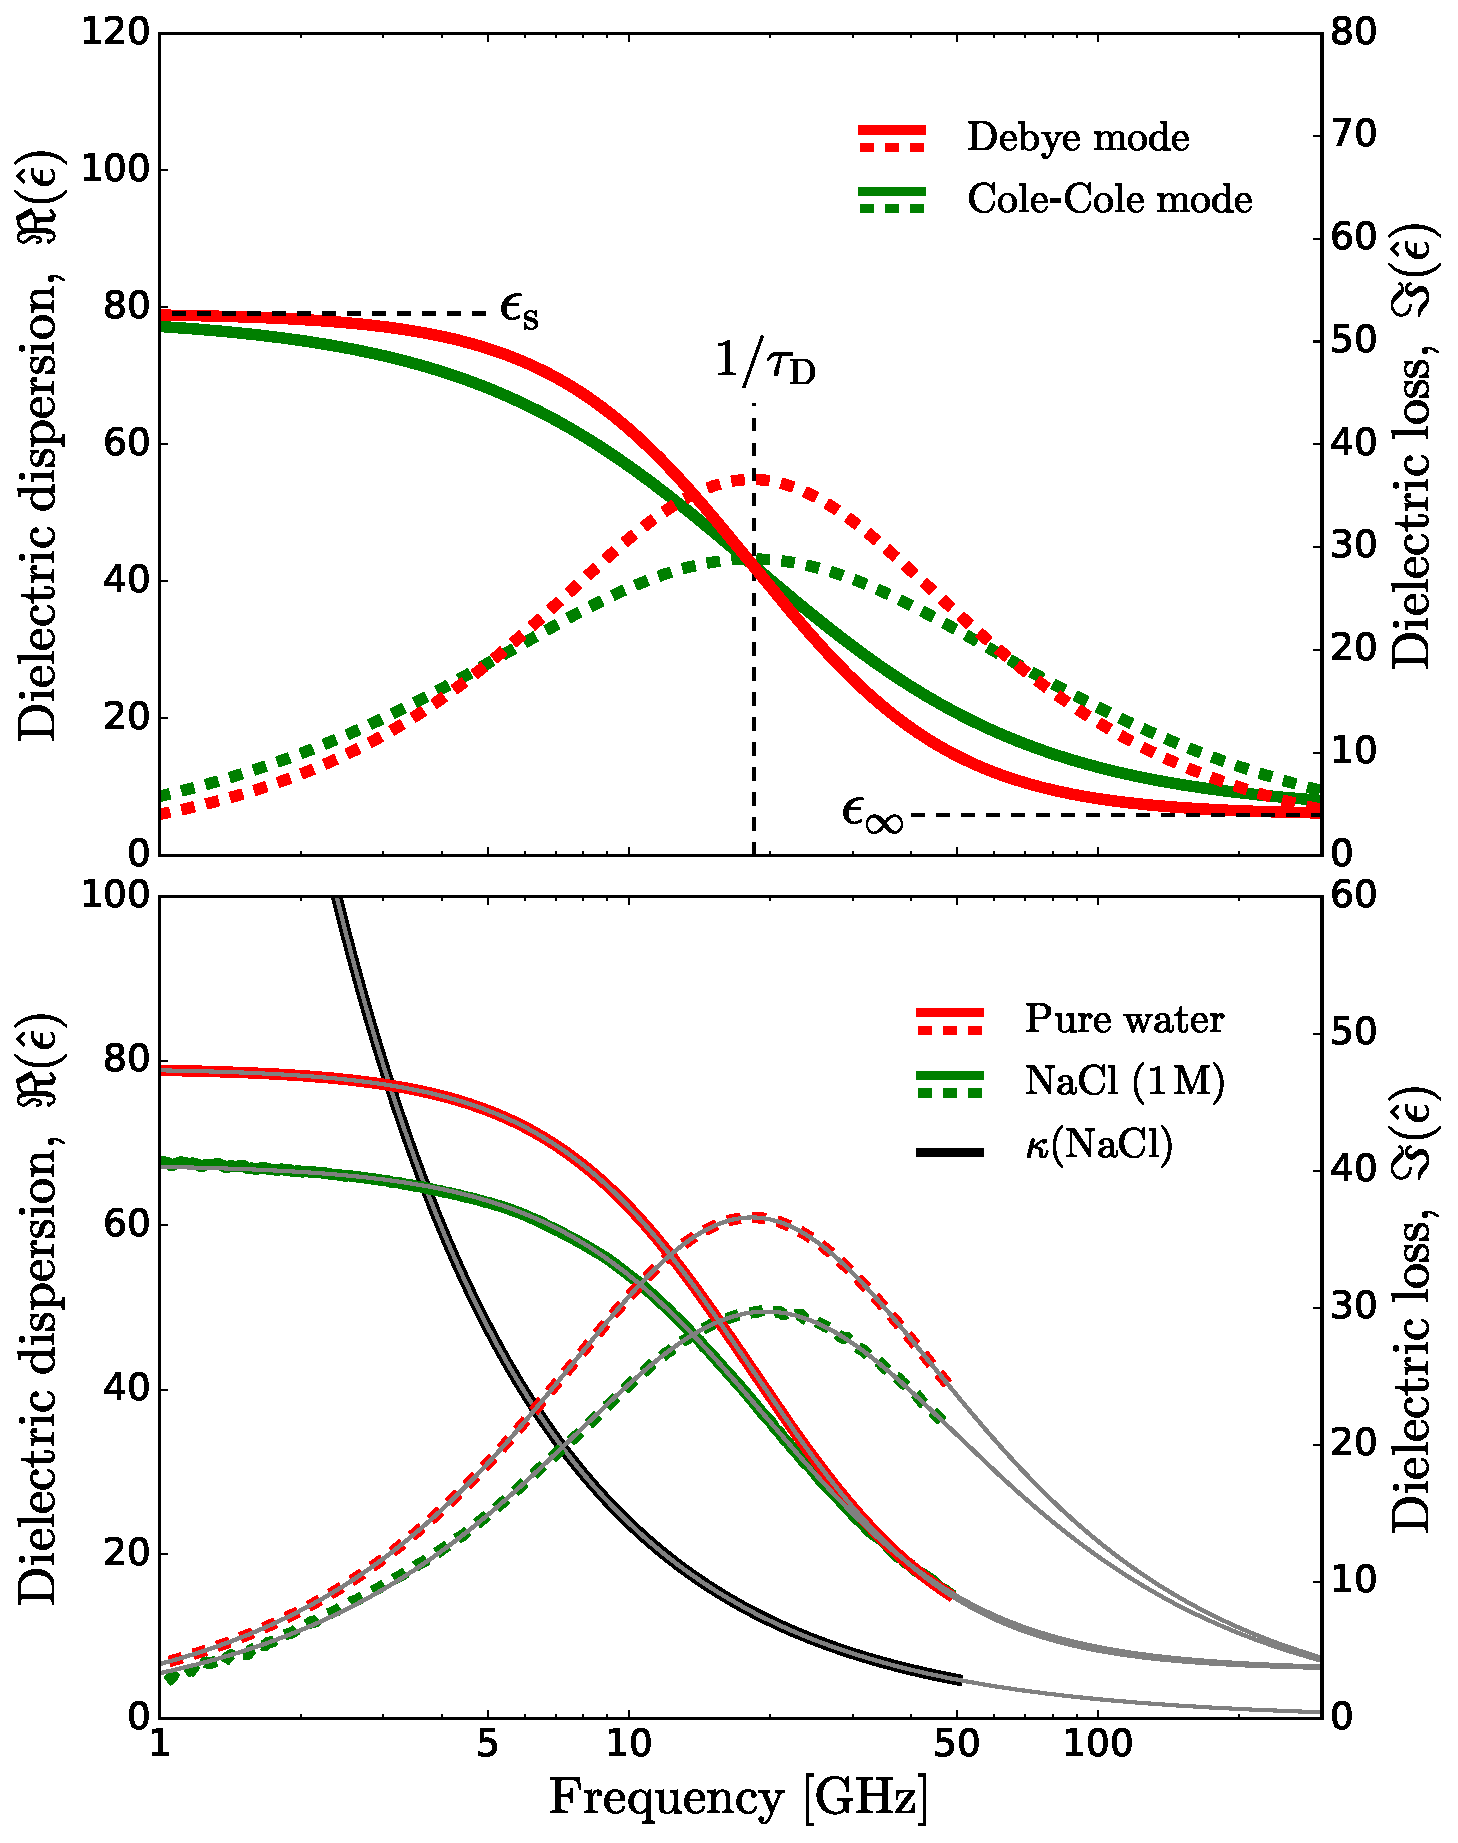
\includegraphics[width=0.85\figwidth]{chapters/Chapter2_Methods/Graphics/DebyeCole_Modes.pdf}
	\caption{The \textbf{upper panel} shows the band shapes of the Debye relaxation mode and the Cole-Cole relaxation mode. In both cases $A_\text{D} = 80$, $\epsilon_\infty = 6$ and $\tau_\text{D} = 8.7$ ps which corresponds to the dielectric properties of pure water at 23$^o$C,\!\cite{Buchner1999b,Ellison1996} while the Cole-Cole deviates from the Debye band by $\alpha = 0.15$. Solid lines represent the dielectric dispersion, and dashed lines the dielectric loss. The \textbf{lower panel} displays dielectric spectra for pure water and a 1 M \ce{NaCl}:\ce{H2O} solution. The corresponding dielectric loss of the alkaline solution has been corrected for the ionic conductivity, which is shown in black. From the dielectric constant at low frequencies, it is clear that the amplitude of the polarization is reduced in the presence of ions, an effect called depolarization. The solid grey curves result from fits using the Debye and the Cole-Cole modes for pure water and the alkaline solution, respectively.}
	\label{RelaxationModes}
\end{figure}


\newpage




For a conducting material, such as electrolyte solutions, the macroscopic dielectric response is modeled with the following generalized permittivity
\begin{eqnarray}
\hat{\eta} (\omega) = \epsilon_\infty + \frac{\epsilon_\text{s} - \epsilon_\infty }{1 + (i \omega \tau_\text{D})^{1-\alpha}} - \frac{i \sigma}{\epsilon_0 \omega},
\label{ColeConRelaxation}
\end{eqnarray}
\noindent which has shown to be sufficient to model the dielectric spectra reported in this thesis. The lower panel in Figure \ref{RelaxationModes} displays dielectric spectra for pure water and a 1 M \ce{NaCl}:\ce{H2O} solution both at 23$^o$C. The Debye mode is well suited to fit the spectra of pure water, while the electrolyte solution is fitted using a Cole-Cole mode showing a broadening of $\alpha = 0.02$. Therefore, the presence of ions induce a relaxation distribution that differs from the single exponential decays.





Moreover, in many systems the dielectric response rises from the contribution of multiple dipolar species, as in aqueous taurine solutions where taurine molecules also align with the electric field,\!\cite{Smit2019} or the discrete dynamics of water in tetramethylurea solutions.\!\cite{Tielrooij2010a} In these cases the dielectric spectrum can be model as the sum of $n$ independent relaxation processes.




\section{Depolarization}\label{SectionDepola}


In electrolyte solutions, ion generate strong local electric fields, orienting the dipoles of neighbouring water molecules. These interactions induce local ordering and reduce (locally) the degrees of orientational freedom of the water, an effect generally called depolarization. This effect reduces the absolute magnitude of the dielectric constant (static permittivity), as is shown in the lower panel of Figure \ref{RelaxationModes}. This depolarization can be described by the sum of three contributions: 

\begin{figure}[t!]
	\centering
	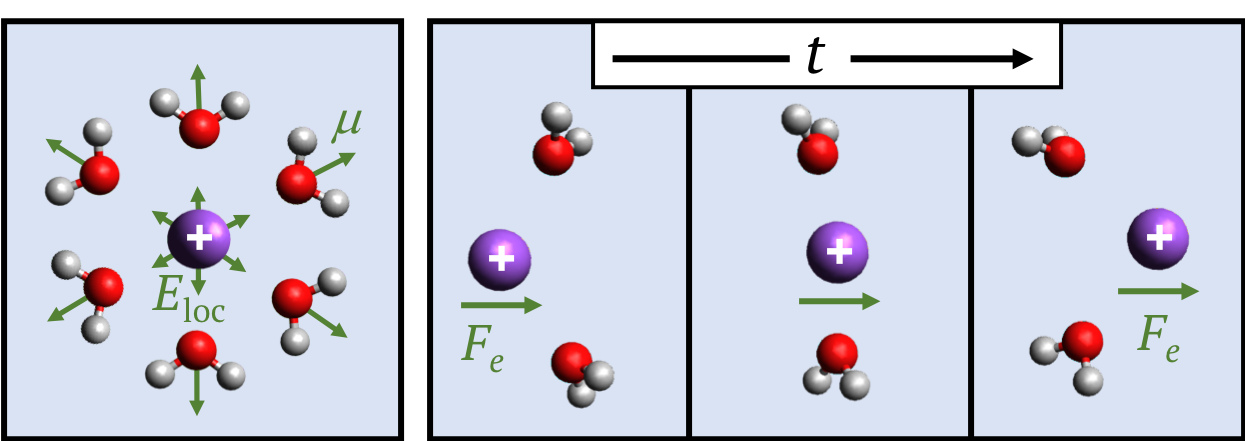
\includegraphics[width=1\figwidth]{chapters/Chapter2_Methods/Graphics/IonicDepolarization.png}
	\caption{\textbf{Left panel:} Static depolarization induces strong binding of water molecules leading to hydration shells. \textbf{Right panel:} Kinetic depolarization rises due to the rotational response of water molecules to the translational motion of ions. Here, $\mu$ is the permanent dipole moment of a water molecule, $E_\text{loc}$ the ionic electric field, and $F_e$ is the driving force that an ion experiences in the presence of a external electric field. The figures are exaggerated representations for conceptual purposes.}
	\label{IonicDepolarization}
\end{figure}

\begin{itemize}
	\setlength{\itemsep}{0pt}%
%	\setlength{\parskip}{2pt}}%
	\item{Dilution of the solvent: having a finite size, the excluded volume of ions leads to reduction in the density of water molecules with respect to the pure solvent.\!\cite{Onsager1936,BOTTCHER1973,Liszi1988} The amplitude of this effect is given by
	\begin{eqnarray}
	A_{\text{D},n} (c) = \frac{c_\text{w} (c)}{c_\text{w,0}} A_\text{D,0} 
	\label{dilutioneffect}
	\end{eqnarray}
	where $c_\text{w,0}$ and $A_\text{D,0}$ are the molecular concentration and the amplitude of the Debye relaxation mode of pure water, and $c$ is the ion concentration. The amplitude of the Debye relaxation mode $A_{\text{D},n} (c)$ scales linearly with the density of water molecules, which is consistent with the Onsager model of Eq.~\ref{KirkFroConstant} since the dielectric response of water is dominated by the reorientation of the dipoles, leading to the approximation that $2 \epsilon_\text{s} + \epsilon_\infty \approx 2 \epsilon_\text{s}$. As a result, the dielectric response $\epsilon_\text{s} - \epsilon_\infty$ of Eq.~\ref{KirkFroConstant} is directly proportional to the density. Eq.~\ref{dilutioneffect} assumes that the dilution does not lead to a change of the Kirkwood correlation factor $g_\text{K}$ of the remaining water in the solution.}
	





	\item{Static depolarization: the strong ionic field induces local ordering in solvation shells, locking the orientational motion of solvating water molecules\!\cite{Impey1983,Barthel1992} (see Figure \ref{IonicDepolarization}). Static depolarization $\Delta A_{\text{D,sta}}$ is linked to ionic hydration numbers\!\cite{Buchner2008} as follows
	\begin{eqnarray}
	Z_\text{hyd} = \frac{c_{w,0}}{A_{\text{D},0}} \frac{\Delta A_{\text{D,sta}} (c) }{c}.
	\end{eqnarray}
	One should take the nature of hydration around cations and anions into account. Static depolarization is generally attributed to cations because they constrain the degrees of orientational freedom of water much more than anions (see Figure \ref{BindingIons}). As such, the relative contribution of the anions to the static depolarization is negligible.\!\cite{Barthel1992,Buchner1999,Impey1983,Guardia1990,Ohtaki1993,Smith1994,Wachter2007}}

	\item{Kinetic depolarization: the long-range orientational response of water molecules to moving ions. An ion moving along the direction of the external electric field causes an opposite orientation of the solvent dipoles as compared to that caused by the external electric field.\!\cite{Hubbard1977a,Hubbard1977,Hubbard1978c,Hubbard1979a,VanderZwan1982,VanderZwan1983a}}
\end{itemize}



\begin{figure}[t!]
	\centering
	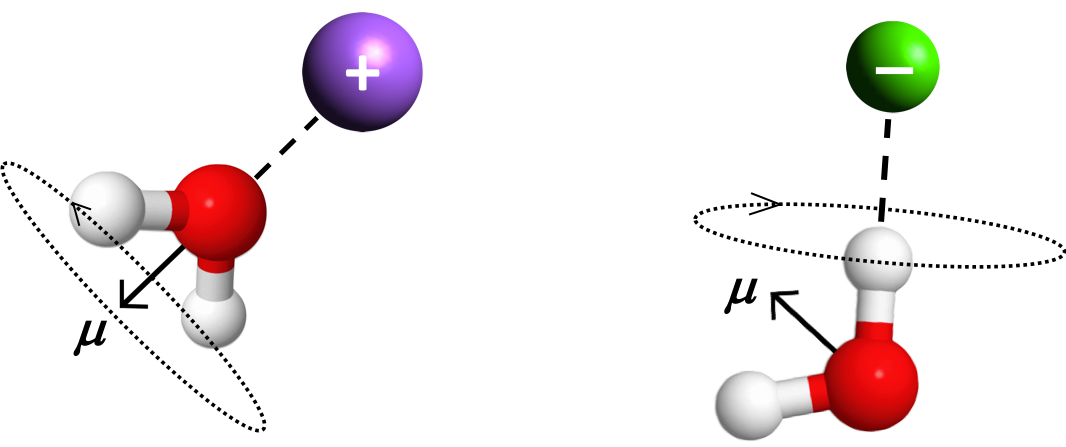
\includegraphics[width=0.7\figwidth]{chapters/Chapter2_Methods/Graphics/BindingIons.png}
	\caption{Static binding in the ionic vicinity. Water molecules hydrating cations are bounded along their dipole symmetrical axis, leading to a negligible orientation motion of the dipole. Hence, water molecules hydrating cations are assumed frozen with respect to the macroscopic dielectric response. On the other hand, water molecules in the anionic vicinity bond along the direction of one of their hydroxyl groups, providing still degrees of rotational motion to the permanent dipole moments.}
	\label{BindingIons}
\end{figure}



The amplitude of depolarization has been widely used to investigate local structuring in solvation shells. However, the static and kinetic contributions are difficult to separate experimentally.\!\cite{Cota2018} Over the last five decades the common approach was to compute the amplitude of kinetic depolarization from theoretical predictions. Hence, the difference between the experimentally obtained depolarization (corrected for dilution) and the value obtained theoretically was assigned to static depolarization, which was used to estimate hydration numbers.\!\cite{Buchner1999,Buchner1999c,Chen2003,Tielrooij2009,Buchner2008,Ensing2013,Sega2014,Ottosson2014c}




The Hubbard-Onsager continuum model for dielectric deficiency\!\cite{Hubbard1977a,Hubbard1977,Hubbard1978c} has been widely used to estimate the magnitude of kinetic depolarization.\!\cite{Hall1981,Nortemann1997,Kaatze1997,Buchner1999,Buchner1999c,Chen2003,Tielrooij2009,Buchner2008,Ensing2013,Sega2014,Ottosson2014c} This model assumes that the ions are immersed in a continuum environment with uniform dielectric behavior as that in pure water. Within this model, it is also assumed that the viscous friction is much larger than the dielectric drag that the orientating dipoles could cause on the ions. Based on these assumptions, the following expression for kinetic depolarization is obtained:
\begin{eqnarray}
\Delta A_{\text{D,kin}} (c) = p \sigma (c)  \left(  \frac{\tau_\text{D}}{\epsilon_0} \cdot    \frac{\epsilon_\text{s} - \epsilon_\infty}{\epsilon_\text{s}}     \right),
\label{HubOnsaKin}
\end{eqnarray}
\noindent where the values between the parenthesis are the dielectric properties of the pure solvent. This equation implies that twater molecules would react to the field of moving ions via a dielectric relaxation mechanism that is the same as the macroscopic dielectric relaxation. 



Hence, changes in the amplitude of kinetic depolarization depend only on the concentration-dependent ionic conductivity $\sigma (c)$, and the factor $p$ that characterizes the frictional forces at the ionic surface. Hubbard and Onsager also derived the values for the $p$-factor, with limiting cases of $p=1$ for a infinite frictional force at the ionic surface (stick) and $p=2/3$ for a negligible friction on the ionic surface (slip). 



It is clear that this model does not account for the ion specificity. In fact, the model implicitly assumes that water preserves the same local structure and ordering regardless the presence of ions, meaning that the cooperative molecular behavior is unperturbed in solvation shells (see Section \ref{KirkFrohSection}).  However, this assumption is contradictory to the notion of ions as structure breakers and structure makers, which have been determined from experiments and simulations.\!\cite{Marcus2009,Shattuck2016} This discrepancy is addressed in Chapter \ref{ChapterPRL}.



\section{Experiment realization}\label{ExperimentalDRS}


Dielectric relaxation spectroscopy enables us to measure the induced complex polarization of a sample in the frequency domain, which in consequence provides the characteristic complex permittivity $\hat{\epsilon} (\omega)$. Vector network analyzers (VNA) are a novel tool to study dielectric properties due to their capacity to measure simultaneously the phase and amplitude of electromagnetic waves in a wide range of frequencies. The used experimental setup is based on a vector network analyzer (Rhode-Schwartz ZVA67) operating at frequencies up to 67 GHz in combination with a open-ended coaxial probe cell. The VNA and the probe cell are connected with a phase-stable coaxial cable (Rhode-Schwartz ZV-Z96). The reflectrometric sample cell is held between two metal blocks that can be set at a desired temperature with a water-flow loop using a thermoelectric chiller (ThermoTek T257P-20) with a temperature stability of 0.1$^o$C.



We perform one-port reflection measurements in which the liquid sample is in contact with the probe head. The reflectrometric disc cell is built based on the probe geometry previously proposed by Blackham et al.\!\cite{Blackham1997} The data are recorded in the frequency range of 1--50 GHz, which encompasses the main relaxation mode of water centered at 18 GHz.\!\cite{Ellison1996}


In this one-port experimental configuration, we applied an initial signal $\hat{a} (\omega)$ to the sample and detect the reflected signal $\hat{b} (\omega)$. These signals are linked via the complex scattering parameter $\hat{S}_{r} (\omega)$ with the following relation
\begin{eqnarray}
\hat{b} (\omega) = \hat{S}_{r} (\omega) \cdot \hat{a} (\omega).
\end{eqnarray}
\noindent where $\hat{S}_{r}$ is related to the dielectric properties of the sample.



In the open-ended probe geometry, the signal is determined by the transition from the impedance of the coaxial probe $\hat{Z}_{c}$ to the impedance of the sample $\hat{Z}_{p}$. The complex scattering parameter is related to the normalized impedance $\hat{Y} = \hat{Z}_p/\hat{Z_{c}}$ via
\begin{eqnarray}
\hat{S}_{r} (\omega) = \frac{1 - \hat{Y} (\omega) }{1 + \hat{Y} (\omega)}.
\end{eqnarray}



\begin{figure}[t!]
	\centering
	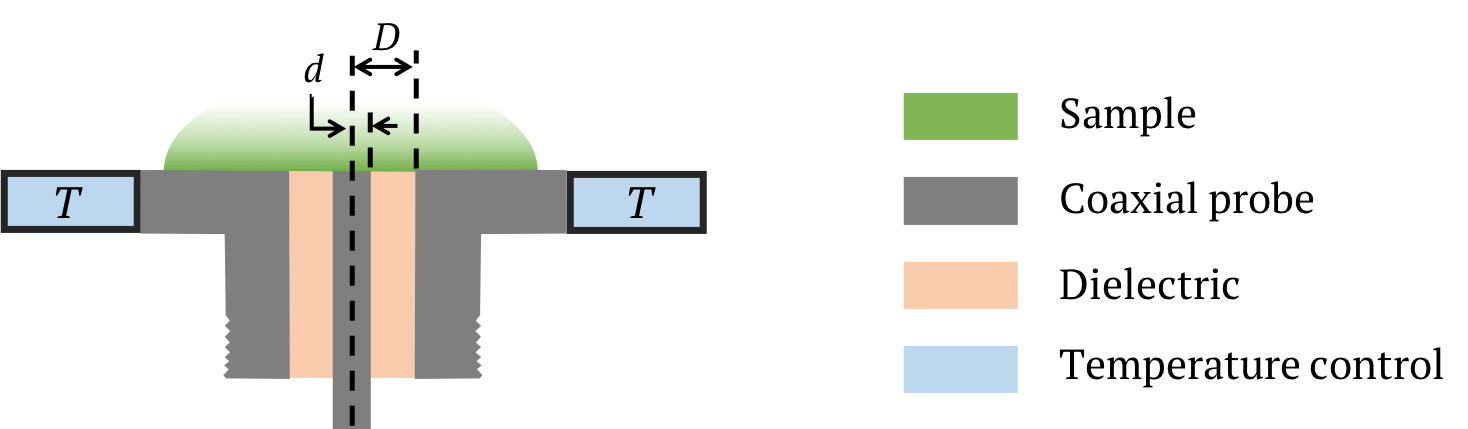
\includegraphics[width=0.8\figwidth]{chapters/Chapter2_Methods/Graphics/SampleCell.png}
	\caption{Transversal cut of the open-ended probe head. The ratio of the incident and the reflected signals at the sample-probe head determines the complex scattering parameter $\hat{S}_r$. The coaxial cable, mentioned in the main text, connects underneath the probe sample cell.}
	\label{SampleCell}
\end{figure}




%Under the knowledge of the probe geometry, a mathematical relation between the complex impedance $\hat{Y}$ and the complex permittivity $\hat{\epsilon}$ can, in principle, be established. Provided with 
For the geometry of the open-ended reflectrometric sample cell, the permittivity-to-impedance relation is given by\!\cite{Blackham1997}
\begin{eqnarray}
\hat{Y} = \frac{ - \hat{k}_s^2}{\pi \hat{k}_c^2 \ln (D/d)} \sum_{n=0}^{\infty} \frac{ (-i)^n \hat{k}_s^{n} I_{n+1}}{n !}
\label{OpenEndedCell}
\end{eqnarray}
\noindent where $D$ and $d$ are the radii of the inner and outer conductors of the coaxial probe, $\hat{k}_c (\omega) = \omega \sqrt{\epsilon_c \epsilon_0 \mu_0}$ is the wavevector of the electric field within the coaxial probe, and $\hat{k}_s (\omega) = \omega \sqrt{\hat{\epsilon}_s \epsilon_0 \mu_0}$ is the wavevector of the electric field in the sample with complex permittivity $\hat{\epsilon} (\omega)$. The coefficients $I_n$ are given by
\begin{eqnarray}
I_n = \int_d^D \int_d^D \int_0^\pi R^{n-2} \cos (\phi) d\phi d r d r' \qquad \text{with} \qquad R^2 = r^2 + r'^2 - 2 r r' \cos (\phi).
\end{eqnarray}



As has been discussed in the original literature for the open-ended sample cell,\!\cite{Blackham1997} the $I_n$ coefficients can be calculated theoretically, but they must be optimized empirically due to the presence of higher order modes of the electric field, which are not included in the derivation of Eq.\ \ref{OpenEndedCell}. The first 40 optimized coefficients $I_n$ have been taken from Johannes Hunger's PhD dissertation,\!\cite{HungerThesis} as have been used for the study of multiple aqueous samples.\!\cite{Hunger2009,Tielrooij2010a,Ensing2013,Ottosson2014c,Cota2018,Smit2019}



Since the sample is located at a certain distance away from the instrument and the setup consist of multiple components, the setup has to be calibrated prior to the measurements. To avoid systematic errors due to imperfections in the electrical network (non-ideal coaxial line), the measured scattering parameter $\hat{S}_{r,m}$ must be corrected to the actual scattering parameter $\hat{S}_{r,a}$ at the probe head according to
\begin{eqnarray}
\hat{S}_{r,m} = \hat{\epsilon}_\lambda + \frac{\hat{\epsilon}_\nu \hat{S}_{r,a}}{1 - \hat{\epsilon}_\sigma \hat{S}_{r,a}},
\label{calibration}
\end{eqnarray}
where $\hat{\epsilon}_\lambda$ accounts for the directional imperfections of the coupling elements, the frequency response $\hat{\epsilon}_\nu$ accounts for changes in the phase that may occur along the finite length of the network, and source match $\hat{\epsilon}_\sigma$ accounts for an impedance mismatch between the the VNA port and the coaxial cable that would lead to re-reflections back to the probe head.



The setup is calibrated by a two-consecutive calibration procedure using three standard references in each step, according to Eq.\ \ref{calibration}. First, the VNA-coaxial cable interface is calibrated via the built-in full-one-port calibration routine using the open, short and match plugs from the ZV-Z218 calibration kit. Second, the interface between the coaxial cable and the sample cell head is calibrated using air (open), conductive silver paint (short) and pure water (match). In all the dielectric relaxation measurements reported in this thesis we employed this calibration routine.



\section{Data analysis and modeling}


Since Eq.\ \ref{OpenEndedCell} has no analytical solution, the complex permittivity is computed numerically via a minimization routine using ``Python'' and the libraries ``Numpy'' and ``Scipy''. These scripts are very extensive to be shown in this thesis, but available at \href{https://github.com/RobertoCota/Dielectric-relaxation-spectroscopy}{https://github.com/RobertoCota/Dielectric-relaxation-spectroscopy}.



The dielectric properties of the solutions studied in this thesis are obtained by means of least-square minimization routines by which the the models discussed in Section \ref{DRTheory} are fitted to the measured dielectric spectra. While the dielectric responses of pure solvents were fitted using a single Debye relaxation mode, the spectra of electrolyte solutions are well described by the sum of a Cole-Cole relaxation mode and a ionic-conductivity term, as expressed in Eq.\ \ref{ColeConRelaxation}. In the lower panel of Figure \ref{RelaxationModes}, the superposed grey lines display the results that best reproduce the experimental data. 



The minimization routine used to determine dielectric properties of electrolyte solutions (as the 1 M \ce{NaCl}:\ce{H2O} in Figure \ref{RelaxationModes}) is shown in Listing \ref{Listing1}.


\newpage


\lstinputlisting[language=Python,caption={Generalized Python script for global analysis in which the real and imaginary components of the complex permittivity are optimized simultaneously.},label={Listing1}]{chapters/Chapter2_Methods/Graphics/OptimizationRoutine.py}





